\section{Computação Paralela}

Com o desenvolvimento da informática em diversos campos houve uma exigência por um maior poder de processamento por parte dos programas. \textit{Softwares} tornaram-se mais sofisticados e computacionalmente mais pesados, assim os processadores começaram a ficar obsoletos face à essa excesso de demanda por processamento. A solução encontrada no início foi acelerar o relógio do processador, porém, com essa aceleração apareceu o problema do superaquecimento desses chips. A solução para esse problema veio com a adição de mais de um núcleo no mesmo \textit{chip}, através da tecnologia \textit{multicore}. Dessa forma, eliminaria-se a necessidade de cada núcleo trabalhar em frequências muito elevadas, tendo somente como base um esquema de escalonamento de tarefas mais eficiente \cite{tanenbaum2013sistemas}.

A ideia desse paradigma de programação é "quebrar" o programa em várias partes e processá-los de forma concorrente (paralela), ganhando assim tempo na execução da tarefa. É interessante notarmos que nem todas as partes de um programa são "paralelizáveis", portanto para esse tipo de aplicação a existência de um ou mais núcleos não resultará na celeridade de sua execução. O paralelismo pode ser explícito quando o próprio programador controla a concorrência ou implícito, quando cabe ao compilador do sistema realizar o paralelismo.

Existem diversos tipos de paralelismo, podermos destacar: 

\begin{itemize}
\item \textbf{No bit}: Nesse tipo dobrava-se o tamanho da palavra (unidade de informação utilizada para cada tipo de computador), com isso dobrava-se a quantidade de processamento por ciclo e consequentemente a diminuição da quantidade de instruções \cite{sriram2009embedded};

\item \textbf{Na instrução}: Assumindo que um programa de computador é constituído por um conjunto de instruções interpretados pelo processador, pode-se combinar essas instruções em blocos que podem ser executados de forma concorrente sem alterar o resultado final\cite{sriram2009embedded};

\item \textbf{No dado}: Geralmente ocorre em laços (\textit{loops}), nas quais uma interação depende de outros resultados\cite{sriram2009embedded};

\item \textbf{No tarefa}: É inerente as aplicações (programas), caracteriza-se ao oposto do paralelismo em dados, ou seja, diferentes cálculos podem ser realizados no mesmo ou em diferentes tipos de dados\cite{sriram2009embedded};

Um ponto crucial para se obter um alto desempenho na computação paralela tange no que diz respeito ao acesso da memória. Existem duas arquiteturas quanto as formas de acesso a memória:

\item \textbf{Centralized Multiprocessor ou Uniform Memory Access Multiprocessor (UMA)}: Nesse modelo as tarefas compartilham de um mesmo espaço de memória e a comunicação é mais simples, pois utiliza-se de uma área comum na memória (Figura \ref{fig_Compartilhada} a);

\item \textbf{Distributed Multiprocessor ou Nonuniform Memory Access Multiprocessor (NUMA)}: Nesse padrão cada processador possui o seu próprio endereço na memória. A comunicação entre esses processadores é feito através de mensagens (Figura \ref{fig_Ditribuida} b). {\color{red} Eu vou concatenar as duas Figuras em uma só. Só não fiz porque ainda não acertei como se faz})
\end{itemize}

\begin{figure}[h]
\center
\subfigure[Memórica compartilhada - UMA]{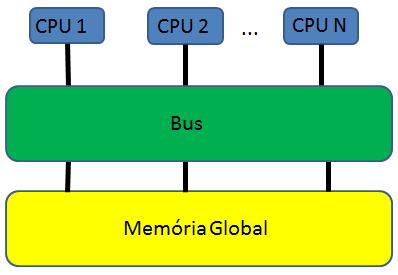
\includegraphics[width=7cm]{figuras/Tipos_Memorias_Shared.PNG}}\label{fig_Compartilhada}
\qquad
\subfigure[Memórica compartilhada - NUMA]{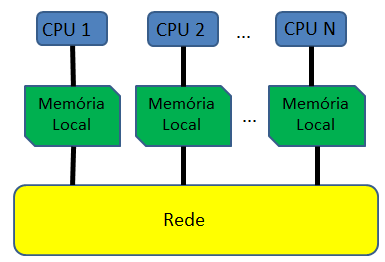
\includegraphics[width=7cm]{figuras/Tipos_Memorias.PNG}}
\caption{Arquiteturas de computação paralela a) Memória compartilhada e b) memória distribuída.}\label{fig_Ditribuida}
\end{figure}


\subsection{OpenMP}

Quanto ao paralelismo, podemos destacar duas formas: o paralelismo explícito e o paralelismo implícito. A seguir destacamos algumas características de cada uma:

\begin{itemize}
\item \textbf{paralelismo explícito}:

\item \textbf{paralelismo implícito}:

\end{itemize}


\subsection{Métricas de desempenho na Computação Paralela}

{\color{red} A idéia aqui aqui é apresentar o/os métodos mai utilizados na avaliação de desempenho quando comparados com a programação sequencial.}





